\documentclass{article}

\usepackage {amsmath}
\usepackage {textcomp}
\usepackage {setspace}
\usepackage [pdftex]{graphicx}
\usepackage[sort&compress]{achemso}
%\usepackage{lineno}

\usepackage[
top    = 0.5in,
bottom = 1.0in]{geometry}
%left   = 2.50cm,
%right  = 2.50cm]{geometry}

% some formatting tags
%\oddsidemargin  0.0in
%\evensidemargin 0.0in
%\textwidth      6.5in

\title{Dancing on Water: The Choreography of Sulfur Dioxide Adsorption to Aqueous Surfaces}
\author{Eric S. Shamay \and Kevin E. Johnson \and Geraldine L. Richmond}

\begin{document}


\newcommand{\suldiox}{SO$_2$}
\newcommand{\ang}{\,$\textrm{\AA}$}
\newcommand{\angs}{\ang}
\newcommand{\wat}{H$_2$O}
%\newcommand{\deg}{$\,^{\circ}$}

\maketitle

%\onehalfspacing
%\linenumbers 
\doublespacing


\begin{abstract}
One might expect the high surface tension of water to be a barrier to absorption of a gas into the liquid phase, but we know that gaseous adsorption onto, and subsequent absorption into a water surface is a common phenomenon on this planet.  What is not commonly known is how an atmospheric gas such as \suldiox~and molecules at the water surface can overcome the barrier created by strong water-water surface bonding interactions.  What this interplay looks like, the distances from the water surface at which these attractive interactions begin, and how they influence the orientational nature of both \suldiox~and surface water molecules is the focus of this computational study.  The results fill a void in the information about this system existing from previous experimental studies by providing information about the dimensional nature of the gas-surface interactions, and the details of how the two species twist and turn orientationally with increased surface interactions.  Classical molecular dynamics have been employed in both equilibrium and steered molecular dynamics (SMD) simulations for \suldiox~at a neat-water surface, and at a surface with high interfacial \suldiox~concentrations.  The results provide new molecular insights for understanding the interaction of this prevalent gas on aerosols and other aqueous surfaces in the environment.
\end{abstract}

\section{Introduction}

Interactions between sulfur species and aqueous systems are the current topic of an active area of research. Sulfur dioxide remains an important industrial product, and also enters the environment naturally through terrestrial processes. \suldiox~acts as a major component of atmospheric pollution, and is a precursor to acid rain formation, and cloud nucleation. Its high solubility in water makes \suldiox~ an integral compound in many atmospheric reactions and surface reaction mechanisms. We seek a fuller understanding of the interactions between \suldiox~and water at interfaces because of the central role \suldiox~takes in many atmospheric particle and aerosol reactions.

Our recent experimental works provided insight into the adsorption and reaction of gases in atmospheric aerosols.\cite{Tarbuck2005,Tarbuck2006} We concluded that an \suldiox~surface hydrate complex forms when an aqueous surface is exposed to \suldiox~gas. A computational study by Dang et al.\cite{Baer2010} then made a series of predictions of the specific nature of the hydrated complex through classical and ab initio simulations. That work developed a detailed picture of the nature of the \suldiox~surface complex with water, and related it to the surface water OH vibrational IR spectra.

Our latest experimental work on \suldiox~behavior further expands our understanding of \suldiox~in atmospheric processes.\cite{Ota2011} A temperature study showed that the binding of gaseous \suldiox~to water surfaces at atmospherically relevant cold temperatures is greatly enhanced. The increased binding facilitates the reaction with water to produce dissolved sulfur species. However, the surface binding of unreacted \suldiox~complexes was found to be a completely reversible process. The same study also showed that low pH aqueous solutions, as often found in atmospheric aerosol composition, inhibit the reaction of \suldiox, but do not affect the surface binding of the gas molecules. The resultant experimental spectra suggest that the surface waters reorient in response to the presence of gaseous \suldiox. From the fitting analysis, one possible geometry of water was posited with the interfacial water ``free-OH'' bonds orienting more perpendicularly to the plane of the aqueous surface. 

In this study we look at the orientational depth profiles of water and \suldiox~during and after the adsorption process. Spectroscopic experiments can not probe depth or orientation profiles of surface species in the same detailed manner as computational simulations. Thus we hope to complement the experimental results of previous studies. We determine the effect of introducing \suldiox~to a \wat~surface, and analyze the orientational response of both the \suldiox~and \wat~molecules using equilibrium and steered (SMD) classical molecular dynamics simulations. The results of this study will help to understand the behavior of adsorbing gaseous complexes, and will verify predictions of our recent experiments. Along with other ongoing experiments and computations, we develop a more complete picture of gaseous adsorption and complex formation on an aqueous surface.

\section{Computational Methods}

Molecular dynamics simulations were performed using the Amber 11 software suite.\cite{Case2010} Polarizable models for the \wat~and \suldiox~molecules were used in the simulations, and have been used previously in studies on interfacial systems because they are known to more accurately reproduce interfacial structure and free energy profiles.\cite{Wick2007,Rivera2006,Dang1998} The \wat~model used is the POL3 water model,\cite{Caldwell1995} and for \suldiox~we used the model of Dang, et al. that places a single polarizable center on the sulfur atom.\cite{Baer2010}

All simulations began with an equilibrated cube of 900 \wat~molecules, with sides of length 30\angs. The long axis of each simulation cell (the axis normal to the water surface) was then lengthened to 120\angs, and the systems were further equilibrated for 10 ns. The simulations all employed periodic boundaries to create an ``infinite-slab'' geometry. After equilibrating the neat-\wat~slabs two types of systems were created by introducing \suldiox: a single-\suldiox~system, herein referred to as the ``neat-water'' system, and a saturated \suldiox~system with multiple gaseous \suldiox~molecules.

The neat-water simulation involved the addition of a single \suldiox~molecule either within the bulk of the water slab (for equilibrium MD), or above the slab surface (in the SMD simulations). The single-\suldiox~system was then evolved for 2 ns to produce an equilibrated starting configuration. The saturated system had 22 \suldiox~molecules in the water slab in order to saturate it to a level coinciding with the Henry's law constant for \suldiox~in water. Additionally, 50 \suldiox~molecules were introduced into the gas phase outside of the water slab, on both surfaces, to simulate an added 50 atm of \suldiox~gas pressure. The saturated system was then evolved for 2 ns to produce a starting configuration for further saturated simulations.

\subsection{Equilibrium Simulations}

Equilibrium simulations involved adding \suldiox~to a water slab and equilibrating as outlined above. One system had a single \suldiox~added to the center of the water box, representing a concentration of 0.06 M. The saturated system with 22 \suldiox~molecules in the bulk represents a system of concentration 1.35 M, with an additional 50 \suldiox~in the gas phase to model 50 atm of pressure above the water surface. Both the low and high concentration systems were then evolved for a further 10 ns using a timestep of 0.5fs, with atomic coordinates written every 100 fs.

\subsection{Steered Molecular Dynamics Simulations}

% need to add in the specifics about the SMD routine, force constants, calculations, etc.
A second set of simulations began with an equilibrated water slab as in the surface equilibrated method above. However, in both the equilibrated neat-water and saturated systems, a single \suldiox~was introduced 20\angs~above the water slab surface, with the sulfur atom tethered to its initial position. The systems were evolved for 1 ns, taking coordinate snapshots every 20 ps to create 50 starting points for further simulations. Steered molecular dynamics (SMD) were then performed on the 50 system configurations (in both the neat-water and saturated configurations) to guide the \suldiox~down towards a tethered water 15\angs~under the water slab surface by applying a small steering force to the \suldiox-sulfur atom.\cite{Isralewitz2001} The \suldiox~thus passed through the continuum of environments from gas phase to (neat- and saturated) water surface adsorption, and finally absorption into the bulk of the \wat~slab. Each of the SMD simulations were performed for a total of 200 ps, using a timestep of 1 fs, and taking snapshots of the system every 25 fs. Figure \ref{fig:starting-configurations} illustrates two sample starting configurations for the SMD simulations, showing both the neat-water slab and the saturated slab configurations before steering the \suldiox~towards the water bulk.

A separate set of SMD simulations were performed with tethering to one of the \suldiox-oxygens. This was done to ensure that the orientation of the \suldiox~during the adsorption transit was not an artifact of the choice of atom used for tethering. The simulations produced the same results (not shown) for the orientational analyses, so the data from the original tethering scheme were used.

\begin{figure}[h!]
	\begin{center}
		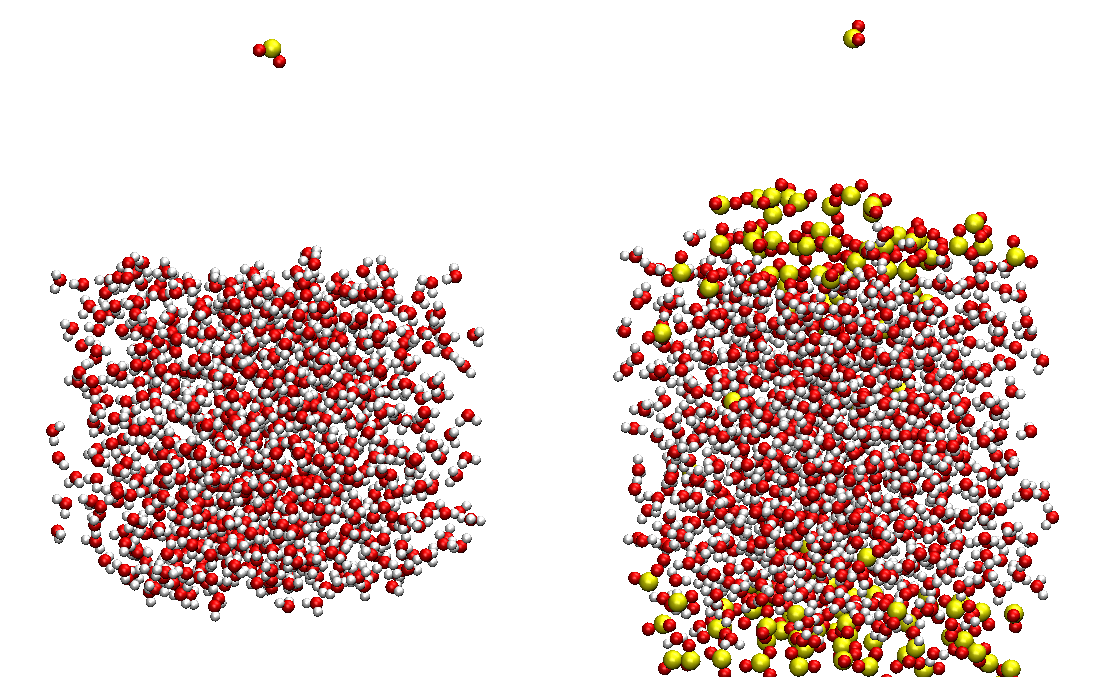
\includegraphics[scale=1.0]{images/startingconfigurations.png}
		\caption{Sample starting configurations for the two types of SMD simulations. The neat-water slab simulation introduces a single \suldiox~molecule that is then guided into the surface of the water and further into the bulk (left). The saturated slab simulation begins with a water system that has been loaded with \suldiox~to saturate the water phase, and also with a high pressure of \suldiox~gas (right). The single \suldiox~(shown at the top) is then steered through the surface region saturated with \suldiox~molecules, and into the water bulk.}
		\label{fig:starting-configurations}
	\end{center}
\end{figure}

\section {Results}

\section{Surface Density Distributions}

One measure of surface activity is the spatial distribution of molecules around the interfacial region. The density distribution of both \wat~and\suldiox~were calculated for the equilibrium MD simulations, and the results are presented in figure \ref{fig:density} for both the neat-water and saturated simulations. The \suldiox~in the neat-water system remained at the top slab surface. While the \suldiox~equilibrated in the saturated system, both in the bulk and gas phases accumulated at both the top and bottom surfaces. 

The density distributions of the \suldiox~were fit to gaussian lineshapes as shown in equation \ref{eq:gaussian} using the common definitions of the variables $A$, $\mu$, and $\sigma$, and given as a function of the distance to the surface, $z$.

\begin{equation}
  \rho(z)=\frac{A}{\sqrt{2 \pi \sigma^2}} e^{-\frac{(z-\mu)^2}{2\sigma^2}}
  \label{eq:gaussian}
\end{equation}

In the neat-water \suldiox~distribution, $\mu=0.781$, $A=0.109$, and $\sigma=1.684$\angs. Thus, the \suldiox~has a surface affinity when in a low-concentration water environment, and it does not fall further into the bulk or move out of the surface into the gas phase. This surface active behavior was found experimentally by a previous SFG study by our group,\cite{Tarbuck2005,Tarbuck2006} and also verified by the computational simulations and spectral calculations of Dang et al.\cite{Baer2010} It was concluded that a surface \suldiox~hydrate complex forms and modifies the structure of water above the Gibbs dividing surface (GDS) shifting \wat~free-OH oscillators in towards the bulk, creating a stronger hydrogen-bonding network. In a later section of this article we look at the effect of \suldiox~on surface water orientation.

Both saturated \suldiox~surfaces exhibit accumulations of \suldiox. However, unlike the neat-water slab, the saturated slab has a non-zero bulk concentration of \suldiox~that does not adsorb to the surface. The coefficient values for the top surface from eq \ref{eq:gaussian} are $\mu_{top}=2.695$, $A_{top}=7.001$, and $\sigma_{top}=3.203$. The bottom surface values are $\mu_{bottom}=-33.846$, $A_{bottom}=6.618$, and $\sigma_{bottom}=3.151$\angs. The added concentration of \suldiox~creates a layer of molecules adsorbed on top of the water surface. The center of this distribution is further into the gas phase than for the single-\suldiox~molecule surface. The accumulation of \suldiox~in this classical simulation coincides with the experimental conclusions of \suldiox~surface hydrate complex formation. However, without simulating breakble bonds the chemistry that may pull \suldiox~into the bulk water phase, and the subsequent reaction to form ions is absent. We have confidence in the surface complexation that is exhibited, the effect of the \suldiox~on the surface water molecules, and the accumulation of \suldiox at the interface. However, we do not yet conclude that the specific locations of \suldiox~on top of the water surface are as accurate as those found in the DFT ab initio calculations of Dang et al.\cite{Baer2010} As was pointed out in their computations, the classical potential does not reproduce the bonding of the first hydration shell around \suldiox, and so conclusions about specific complex formation or geometries are best made from the ab initio simulation results reported.

\begin{figure}[h!]
	\begin{center}
		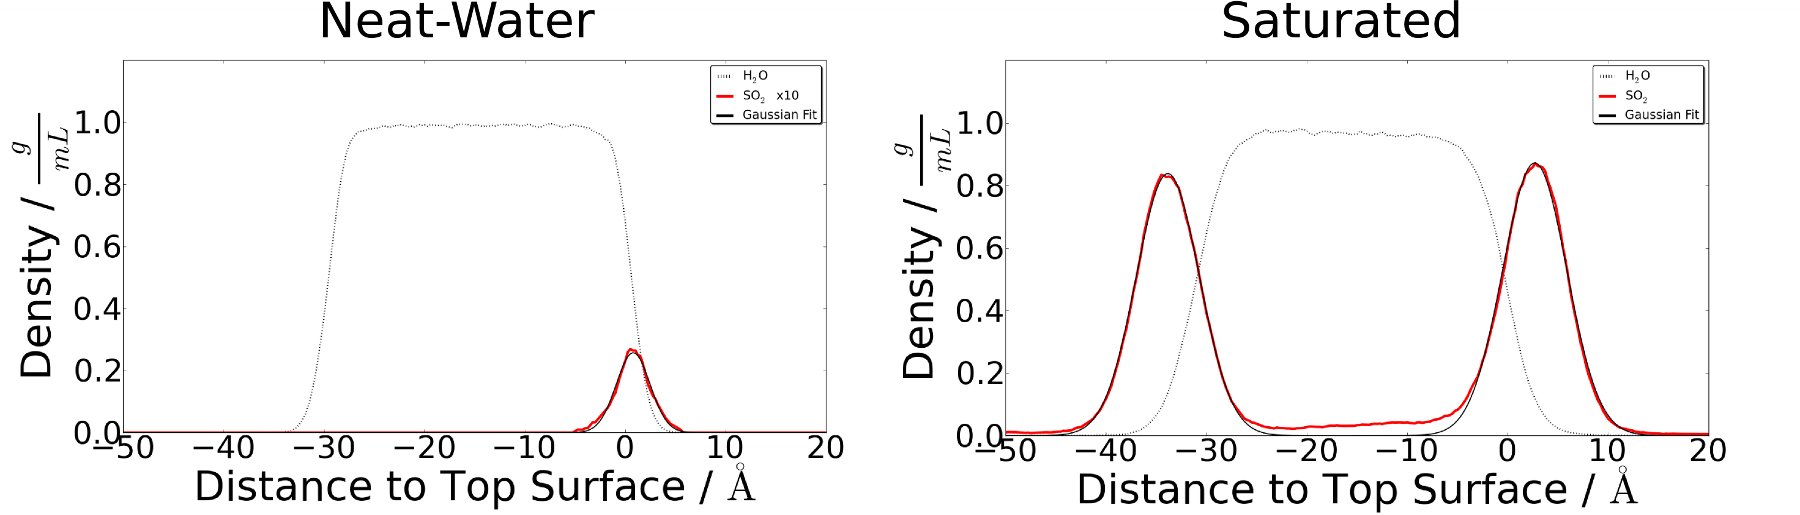
\includegraphics[scale=1.0]{images/density/density.png}
		\caption{Molecular density distributions of \wat~and \suldiox~calculated along the long-axis of the simulated cells. The distance axis shows the distance of the given molecule from the top surface of the \wat~slab, with positive values located above the slab towards the gas phase, and negative values located in the water bulk. The lower slab surface is located at approx. -30\angs. Distributions of both the neat-water simulation with a single \suldiox~(left, scaled 10x for clarity), and the saturated system (right) are shown.}
		\label{fig:density}
	\end{center}
\end{figure}

\subsection{Equilibrated MD}

Geometric analyses were performed to characterize the net molecular orientation of \wat~and \suldiox~molecules at different depths from the water surface location. At each distance from the surface location, an orientation profile was created for both the \wat~and \suldiox~molecules. The orientation distribution for the angles $\theta$ and $\phi$ at all depths were combined to form 2D intensity plots that show how the molecular orientation distributions change with distance to the surface location. These plots (Figures \ref{fig:water-orientation}, \ref{fig:so2-transit-angles}, and \ref{fig:so2-surface-angles}) allow for a visual interpretation of how the net orientations are affected when moving from the gas phase through the interfacial region and to the surface location, and then further into the aqueous interfacial region and bulk. Both the neat-water, with only a single \suldiox~introduced, and the high-concentration saturated system were analyzed. In the case of the neat-water system, the introduction of a single \suldiox~does not greatly affect molecular orientation of water molecules in the interfacial region. These results of the water orientation are very similar to a neat-water system without any adsorbed solutes (not shown).

The 2D orientational depth profile plots show areas of low intensity in dark blue, and highest intensity in dark red. Regions of the plots where the intensity (coloration) is equally distributed from top to bottom along the entire orientational range are considered isotropic. Likewise, areas of the plot with high intensity over a small orientational range are considered to exhibit an orientational preference at the given depth.  The histograms are arranged with the plots of $\cos(\theta)$ on the left and $\cos(\phi)$ on the right. The surface is located at 0\angs. The angle distributions from both simulated slab surfaces were averaged for all the orientation analyses.

\subsubsection{\wat~Orientation}

The orientation depth-profiles for \wat~are shown in Figure \ref{fig:water-orientation} for both the neat-water (top) and saturated (bottom) systems during the equilibrium MD simulations. The interfacial region for both these calculations and the VSF experiments is defined as the region where molecular orientational anisotropy exists around the surface water location. Referring to Figure \ref{fig:water-orientation}, calculations indicate an interfacial width of approximately 10\angs~for the neat-water system, and approximately 16 \angs~for the saturated system. In both systems the strongest orientational preference is found at the slab surfaces (positions above 0\angs) where the water is furthest towards the gas phase. Previous work on orientational preference of water at air surfaces shows the same trend as our neat-water results.\cite{Walker2006b,Hore2008} The narrow "peninsula" of high intensity that extends in the $\cos(\theta)$ plots to the right of the -5\angs~location shows the overall preference of water to orient at the surface. The $\cos(\phi)$ plots are similar to each other with a narrow region of reorientation, but the effect in the interfacial region is greater in the neat-water system as evidenced by the sharper transition in intensity from blue to red, compared to the saturated system that has a less pronounced intensity change.

The bisector tilt of the water molecules, $\cos(\theta)$, concentrates around $\cos(\theta)=0$ within the first few\angs~above and below the water surface location, becoming progressively isotropic further through the interfacial region and into the water bulk of both systems. As the tilt nears $\cos(\theta)=0$ the \wat~bisector lies within the plane of the surface indicating a water orientation either flat on the surface, or with some amount of ``twist'' sending the OH bonds in towards, or out of the bulk. The value of $\phi$ determines the ``twist'' in this case. Both systems show a defined intensity concentration (dark red) in the distributions around $\cos(\phi)=1$ on the aqueous side of the interfacial region. This results from an orientation of the water's y-axis (normal to the molecular plane) aligned perpendicular to the plane of the water surface. Thus, for both the neat-water and saturated systems, the preferred orientation of water molecules at a distance of 0\angs~ is to lie mostly flat to the plane of the interface with a slight ``twist'' sending one OH bond further into the gas phase, and the other OH towards the water bulk. This result agrees somewhat with a recent air/water study by Fan et al. in which the surface orientations of several water models were analyzed.\cite{Fan2009} They simulated water using non-polarizable models, however, which alters the behavior of water at interfacial regions when compared to the polarizable POL3 model used in our work. The main conclusions are similar in that one OH tends to point further into the air phase than the other, but differs in that this effect is less pronounced with the polarizable model.

Although the plots show overall similarities for both the neat-water and saturated systems, the presence of a layer of adsorbed \suldiox~molecules alters the orientation of those waters furthest into the gas phase. For the saturated solution the resulting orientation of waters above 0\angs, shown in the saturated plot of $\cos(\theta)$ of Figure \ref{fig:water-orientation}, is with a bisector pointing further into the adsorbed \suldiox~gas layer, and both hydrogens pointing outward from the aqueous bulk. The effect is more pronounced further from the water phase, and above 5\angs~the $\cos(\theta)$ distribution is completely centered around $\cos(\theta)=+1$ (see Figure \ref{fig:water-angles}).

%The histograms show overall similarities for both systems in their shapes and intensities from approx. 0\angs~and below. The presence of a saturated layer of adsorbed \suldiox~molecules, however, alters the water orientation, but not necessarily the orientational depth of the interface. In both $\theta$ distributions, the orientations of waters in the bulk region are isotropic until 5\angs~below the surface location. At 5\angs~below the surface the water molecules begin to orient with their bisectors within the plane of the interface (perpendicular to the surface normal, $\cos(\theta)\approx 0$). The corresponding location in the plot of $\phi$ shows that those molecules are also mostly flat to the surface ($\cos(\phi)\approx 1$). Moving further out from the bulk and into the gas phase, the distributions show $\cos(\theta)$ increasing. Waters further out from the bulk have fewer bonding interactions, and orient with their hydrogens more towards the gas phase. The bisector pointing further into the gas phase leads to isotropy in the values of $\phi$.  

The noise in the neat-water plots of Figure \ref{fig:water-orientation} above 5\angs~(manifested as disconnected points of intensity throughout the range of orientations) is a result of fewer waters venturing beyond those extents and thus less data far from the water surface location. This is one indication that waters near a layer of adsorbed \suldiox~venture further above the interface relative to the low \suldiox~concentration, where they can have more \suldiox~interaction with the adsorbed gas molecules. These results show that the interactions with neighboring \suldiox~molecules allow the waters above the surface to orient more perpendicularly to the interface. This is consistent with our recent experimental VSFS studies which showed evidence for the reorienting behavior of water due to the \suldiox~interactions with the topmost surface waters.\cite{Ota2011}

The distribution of $\cos(\phi)$ is more sharply defined (i.e. less isotropic) for the neat-water system than for the saturated one. Waters on the neat surface lie flatter, whereas the presence of the \suldiox~allows a greater range of ``twist'' for those waters in the plane of the interface. The $\phi$ distributions quickly become isotropic above the surface as the bisectors orient more perpendicularly, and below the surface as the bulk water loses any orientational preference.

%Peaks in the distributions of the neat-\wat~system are more clearly pronounced as their intensities are more concentrated and larger than the surrounding area of the profiles. This difference indicates that the transition from the preferred orientation at the water surface has a sharper distinction from the isotropic bulk than in the system with the saturated \suldiox~surface. It appears that the same orientation trend is present in both systems, but the presence of the \suldiox~at the water surface decreases the degree of water orientation at the interface.

\begin{figure}[h!]
	\begin{center}
		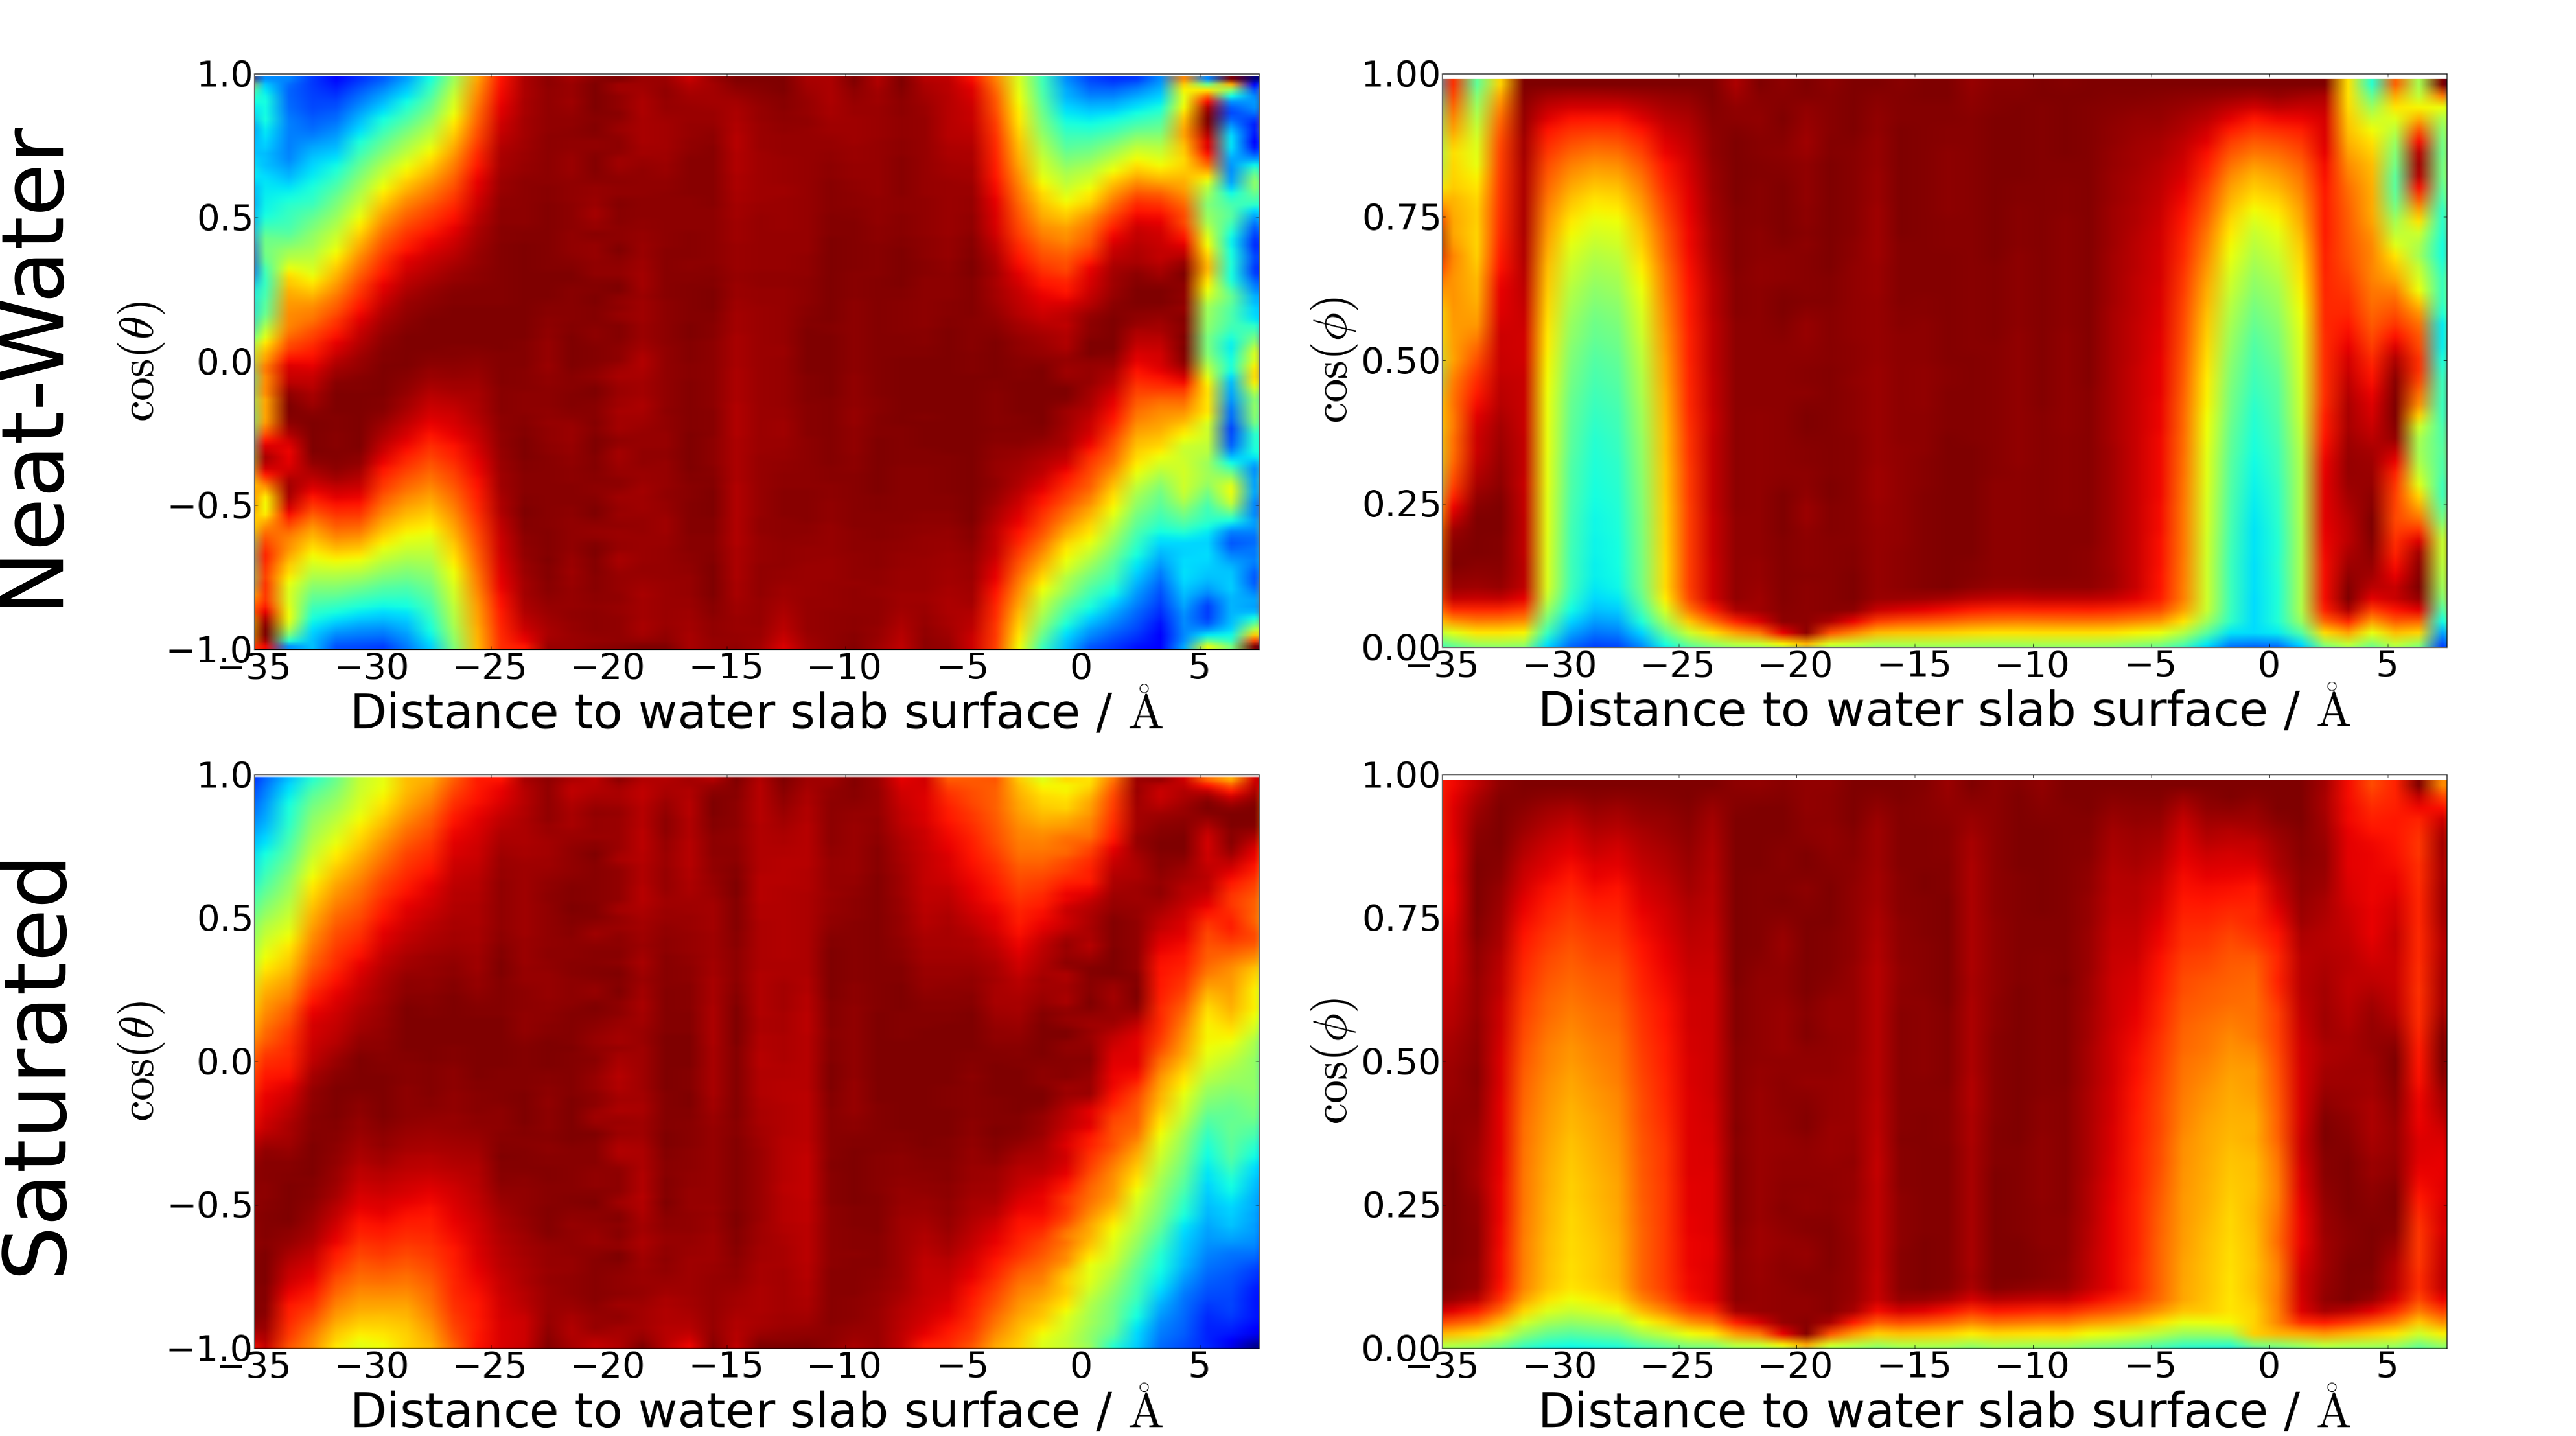
\includegraphics[scale=1.0]{images/h2o-angles/h2oangles.png}
		\caption{Molecular orientation histograms of \wat~throughout the surface equilibrated systems. The top surface is located at a distance of 0\angs~with negative distance values located in the bulk of the slab. Shown are the angle distributions for $\theta$ (left column) and $\phi$ (right column) in both the neat-\wat~system (top row) and the saturated system (bottom row). The distributions are normalized to account for the changing number of water molecules at different positions in the system. Regions of high intensity are dark red, and low intensity are dark blue. The scattered points of coloration to the far right of each plot indicates that few waters were located at those positions, and thus few data points were collected.}
		\label{fig:water-orientation}
	\end{center}
\end{figure}


\subsubsection{\suldiox~Orientation}

Orientation distributions of the adsorbed \suldiox~molecules were created during the equilibrium simulations for both the neat-water and saturated systems. Figure \ref{fig:so2-orientation} shows the distributions of $\cos(\theta)$ and $\cos(\phi)$ (arranged similarly to the water orientation distributions plots in Figure \ref{fig:water-orientation}). The \suldiox~orientation data set for the neat-water system is much smaller as only a single \suldiox~molecule was simulated in the bulk. The resulting distribution plots are thus noisier than the corresponding saturated plots with more scattered points of high intensity, but effective comparisons can still be drawn.

In the interfacial region within 0-5\angs~of the water surface location (the approximate distance from the surface that \suldiox~begins interacting with the outer-most waters) the angular distribution of the single \suldiox~(in the neat-water system) is concentrated primarily in $\cos(\theta)>0$. The peak of the distribution occurs at $\cos(\theta)=1$. This indicates that the \suldiox~bisector points out of the water surface, with the sulfur atom pointing towards the aqueous bulk, and the two oxygens pointing into the gas phase. This same distribution occurs in the saturated system for positions below 5\angs. Beyond 5\angs~above the surface both distributions become isotropic. Promixity to the water highly orients the \suldiox~with the sulfur atom pointing in towards the water bulk. Moving further away from the water surface, and interacting less with \wat~molecules allows for greater orientational freedom as exhibited in the isotropy of the distributions above 5\angs. %Because both the neat-water and saturated systems show rather similar distributions, it is possible that the concentration of \suldiox~does not strongly affect the orientation of the \suldiox, unlike the orientations of waters.

The plots of $\phi$ are both isotropic, although the neat-water system plot is quite noisy from the small data set. Because the \suldiox~near the surface is oriented perpendicularly to the interface, the $\cos(\phi)$ orientation is expected to be isotropic. Further from the water surface where the bisector orientation becomes isotropic, the $\cos(\phi)$ distribution also becomes isotropic. For the \suldiox~orientation, the $\phi$ angle does not provide further information regarding the surface behavior.

The plots indicate that \suldiox~orients similarly at both the low and high concentration interfacial environments. The plots of $\phi$ for both concentrations exhibit isotropic distributions. However, the $\theta$ values follow similar trends at both concentrations indicating that the \suldiox~sulfur orients down towards the water phase, with both oxygens pointing away from the surface once the \suldiox~is within approx. 5\angs~of the surface. This behavior continues down to at least 5\angs~below the water surface location, notwithstanding any chemical reactions that may occur that are not simulated using the classical MD techniques utilized in this work.

\begin{figure}[h!]
	\begin{center}
		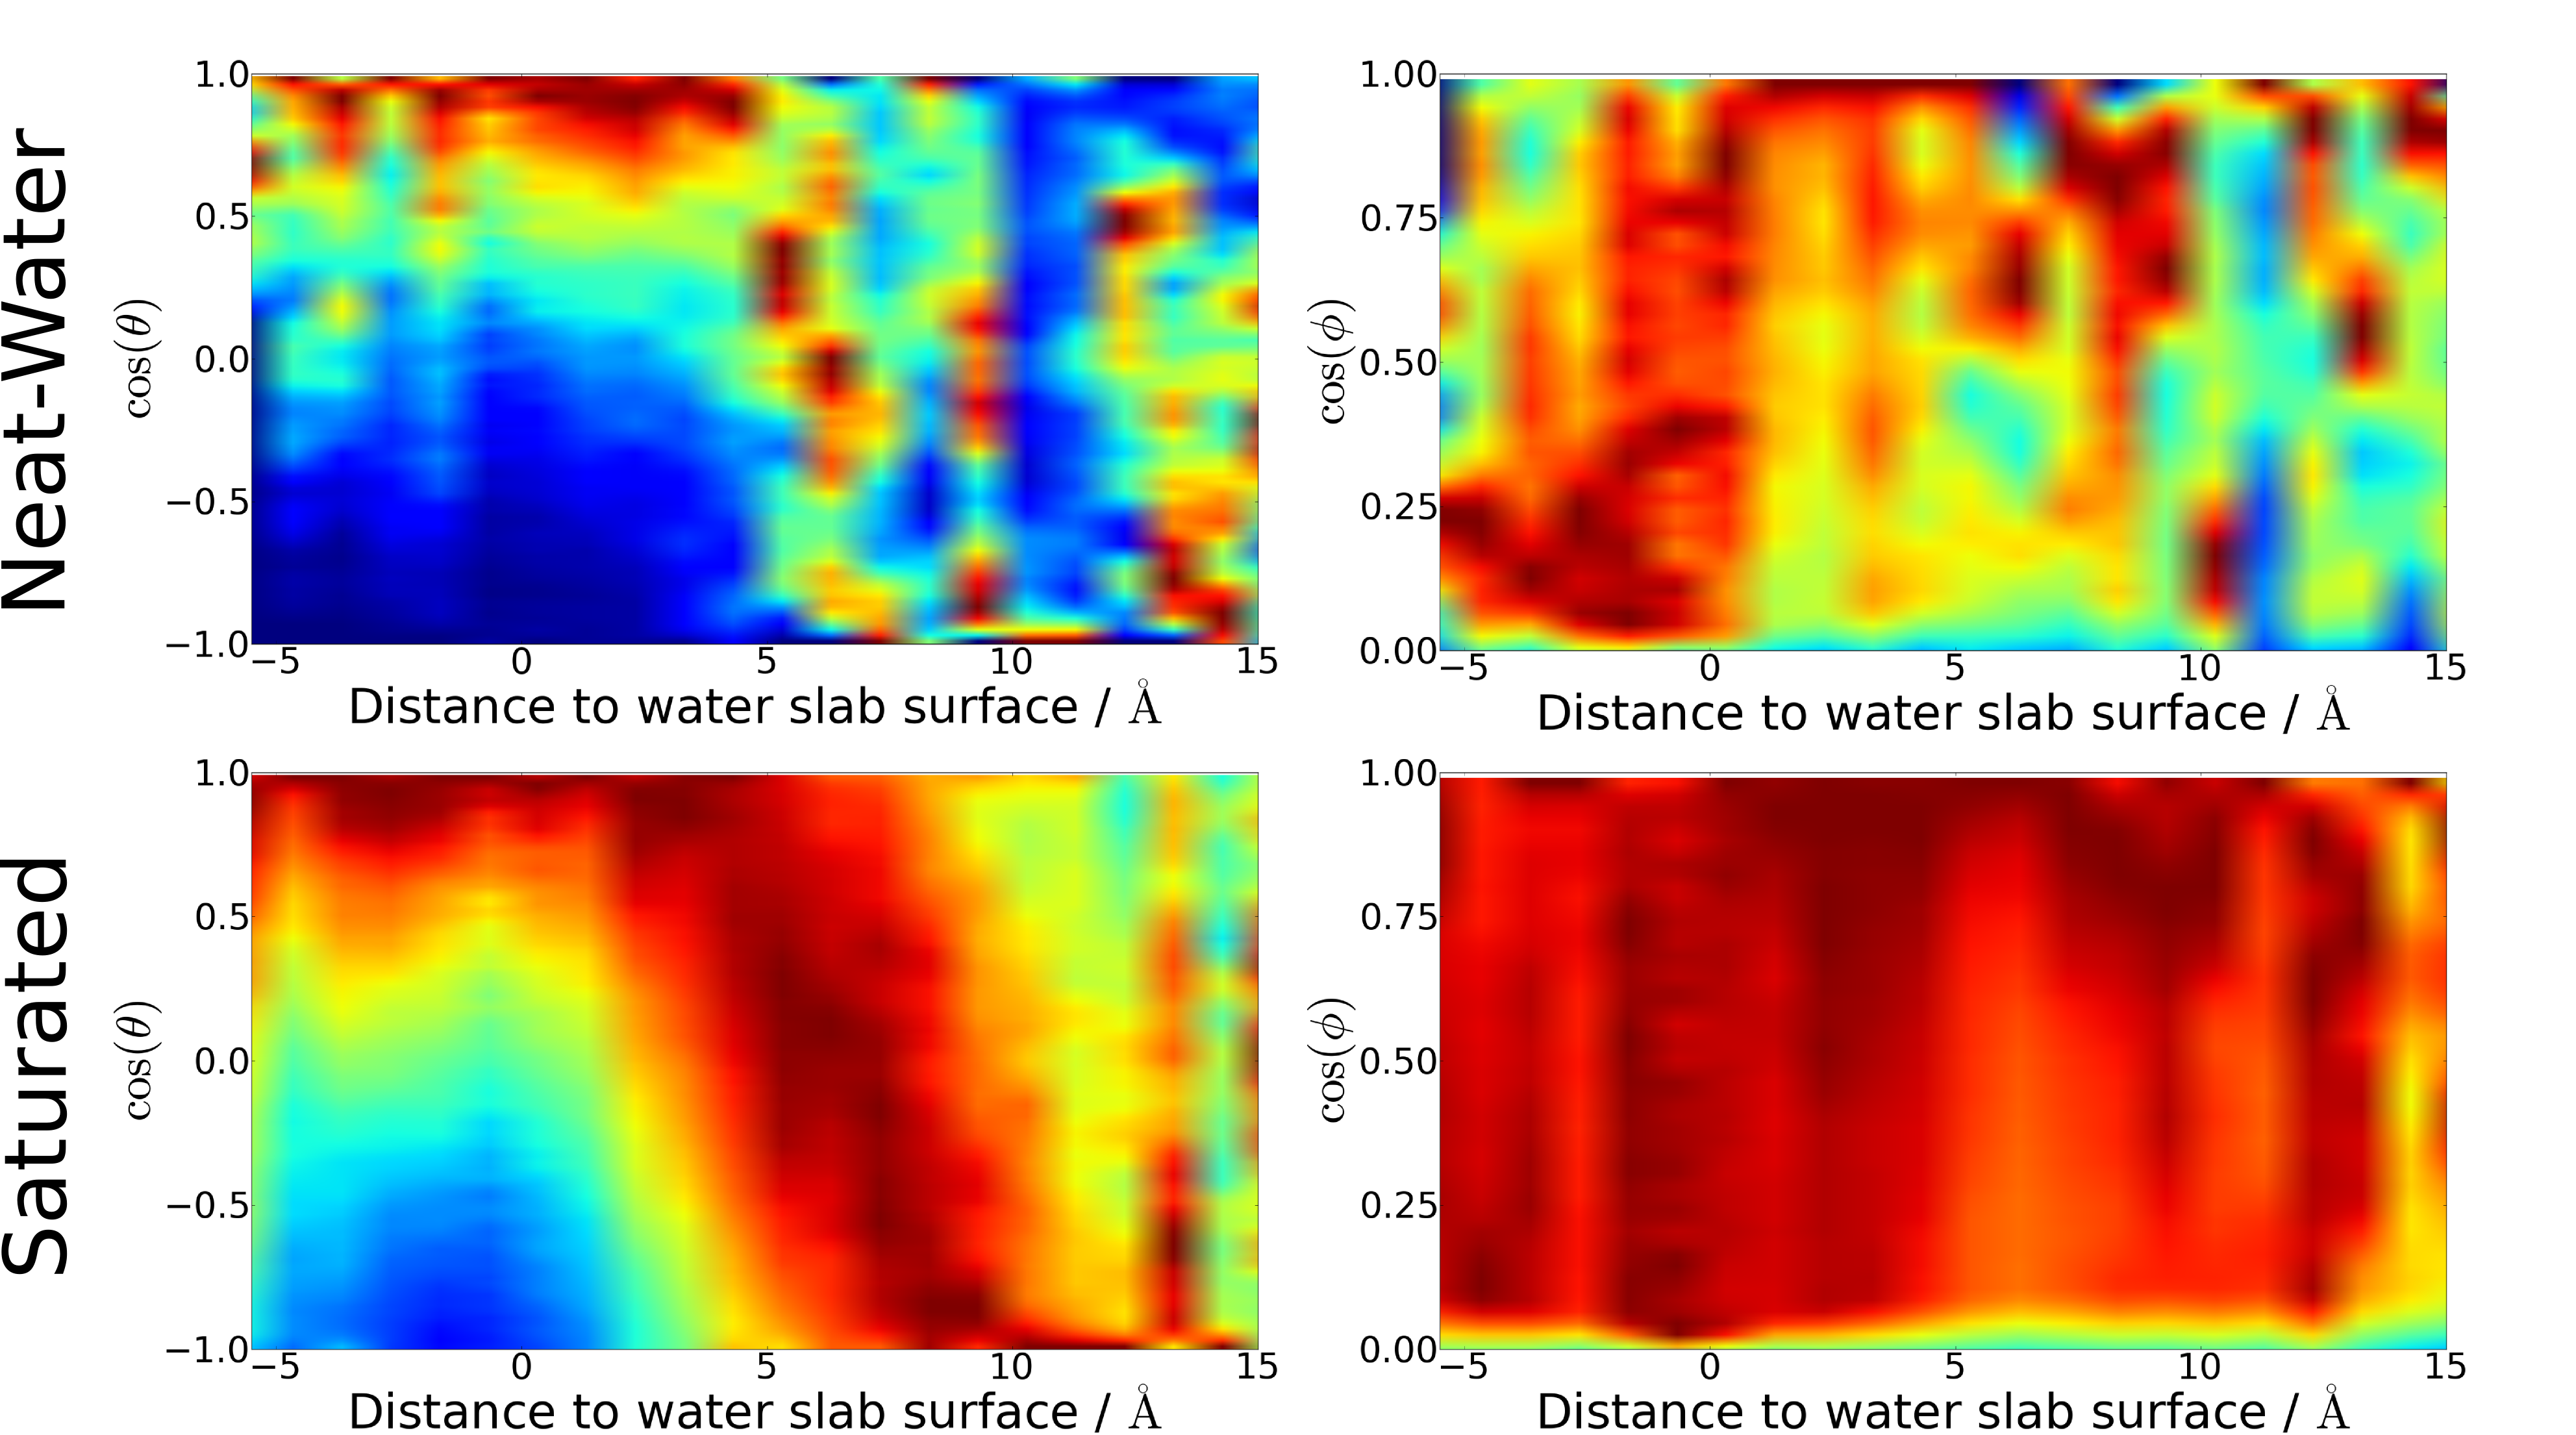
\includegraphics[scale=1.0]{images/so2-angles/so2-angles.png}
		\caption{Molecular orientation distributions for \suldiox~molecules adsorbed to the water slab surface. Distributions are shown for $\cos(\theta)$ (left column) and $\cos(\phi)$ (right column) for both the neat-water (top) and saturated (bottom) systems. For both systems the $\theta$ distributions show \suldiox~bound to the water surface with the sulfur pointing towards the water slab, and the oxygens pointing to the gas phase. In this configuration the $\phi$ distribution is isotropic because of the water slab's in-plane symmetry.}
		\label{fig:so2-orientation}
	\end{center}
\end{figure}

\section{Steered MD Transit Simulations}

\subsection {\suldiox~Orientation}

	The orientation of a \suldiox~molecule adsorbing to an aqueous surface was determined through an analysis process to find the angles $\theta$ and $\phi$ (figure \ref{fig:water-angles}). For each timestep of the SMD simulations the orientation angles were determined for the transiting \suldiox~as it was pulled into the water slab from the gas phase, both in the neat-water and saturated slab systems. The angle cosine values were collected for the 50 simulations for both systems, and the binned with the position of the \suldiox~relative to the water slab surface location. The resulting 2-dimensional histograms shown in figure \ref{fig:so2-transit-angles} show the orientation trend for the \suldiox~in the gas phase (above 0\angs), near the aqueous surface (near 0\angs), and after entering the water bulk (below 0\angs). Only the surface into which the transiting \suldiox~was steered is shown for the saturated system.

\begin{figure}[h!]
	\begin{center}
		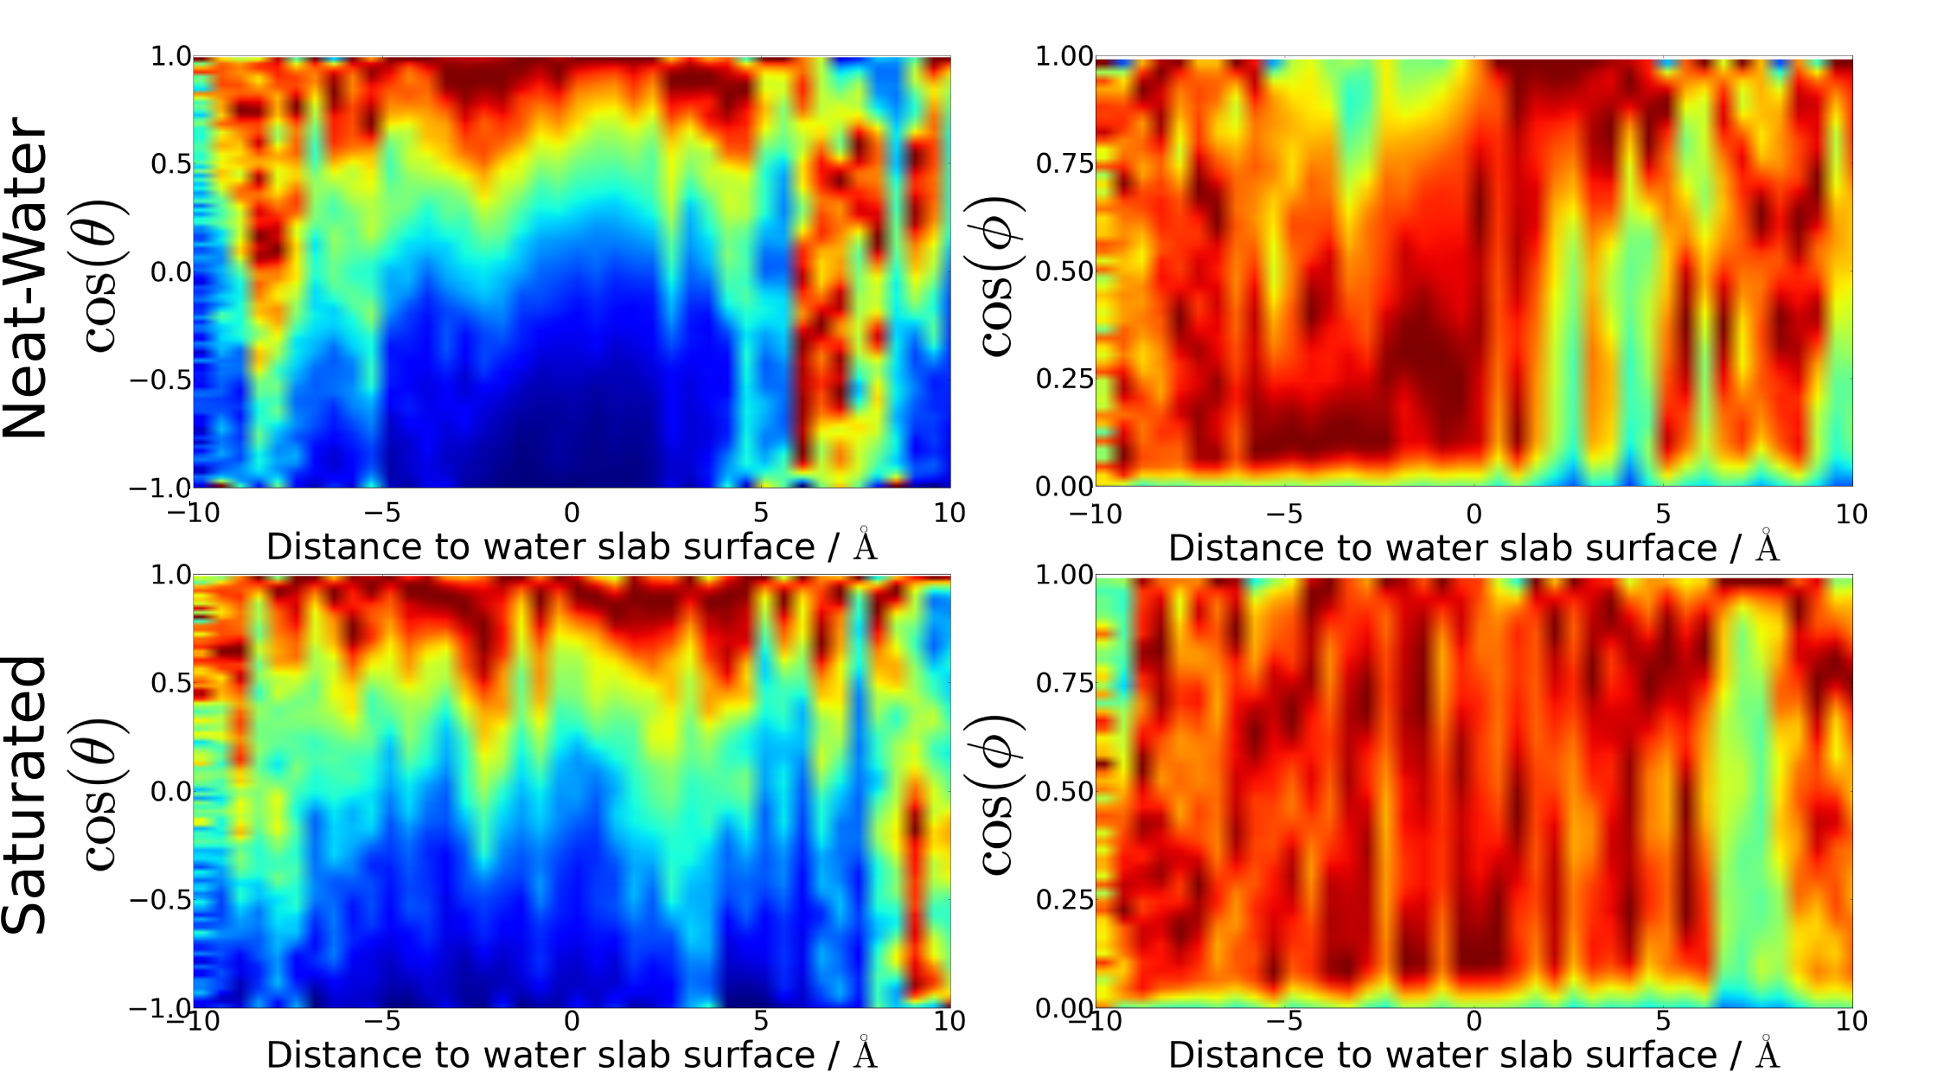
\includegraphics[scale=1.0]{images/transit-so2-angles/so2-angles-transit.png}
		\caption{\suldiox~molecular orientation distributions during SMD transit simulations into an aqueous slab. Both the neat-water (top row) and saturated (bottom row) data sets were analyzed to determine the angles $\theta$ (left column), and $\phi$ (right column) of the transiting \suldiox. The distributions show angle cosines plotted against the distance of the \suldiox~to the location of the water surface. The data sets were averaged at each distance for the respective 50 simulations.}
		\label{fig:so2-transit-angles}
	\end{center}
\end{figure}

	%From its starting position 20\angs above the water surface, until the \suldiox~moves to within 5\angs of the surface of both systems, the orientation is isotropic in both $\theta$ and $\phi$. Upon approaching the saturated surface at approx. 5\angs, the \suldiox~$\phi$ orientation distribution begins to cluster near $\cos(\phi)=1$, with the $\theta$ distribution remaining more isotropic, but with a trend of $\cos(\theta)>0$. At 5\angs the \suldiox~begins interacting with the other \suldiox~molecules that sit atop the water, and the resulting orientation distribution suggests that contact with the \suldiox~layer causes the adsorbing molecule to lie more flat to the surface. Within this same region from 0-5\angs above the surface, the $\phi$ distribution of the neat-\wat~system remains isotropic. The intensity of the distribution (darker blue) also indicates that the \suldiox~spends little time in this region, as it is quickly adsorbed further into the water bulk.

	%Just below the water surface as the distance moves into negative values, both systems show clear orientational preferences. In both systems the bisector orientation clusters such that $\cos(\theta)<0.5$, with most of the distribution intensity around $\cos(\theta)=1$. This suggests that \suldiox~in a water surface orients with the sulfur pointing into the water bulk, and the oxygens pointing towards the surface water molecules.

	%Differences occurr between the system orientation profiles once the \suldiox~has moved further than 10\angs below the surface. While both $\theta$ and $\phi$ hold the same trend from just under the surface through to the bulk of the slab in the saturated system, the orientation profile becomes much more isotropic past 10\angs under the surface of the neat-\wat~system. The orientation effect is shallower under the neat-\wat~surface. However, the orientation distribution peaks most intensely, and more tightly clustered with the \suldiox~bisector aligning with the surface normal, just underneath the neat-\wat~surface than the saturated one. The distributions thus show an orienting force extending deeper into the surface of the saturated system than the neat-\wat~system. In terms of how deeply the \suldiox~molecule is oriented, the interfacial region of the saturated system is larger and extends further into the aqueous bulk.


\section {Conclusions}

Gaseous adsorption on solid surfaces has been extensively studied over the past few decades with much learned about how molecular geometry and orientation of the adsorbate are influenced by the proximity of the solid slab.  For a liquid surface where the surface slab is no longer rigid but has molecules with considerable freedom of movement, the surface and approaching gas molecules can be active partners in attaining the optimal geometry and orientation necessary for adsorption and subsequent uptake.    And unlike the solid surface defined by a sharp plane, the interfacial region for the liquid-gas system is much broader, extends on either side of a defined center plane, and is host to a broad distribution of gas-liquid molecular geometries and orientations that change as the gas molecules transit through the interfacial region into the bulk liquid.  Although  our current molecular level understanding of  the complex dances that these molecules play in this fluid interfacial region is in its infancy, emerging studies such as these are beginning to provide unique new insights that are key to understanding many  environmentally important processes at aqueous surfaces.

Presented herein are the results of several classical molecular dynamic simulations that focus on understanding how surface water molecules and adsorbing \suldiox~gas molecules twist and turn as the gas transits the interfacial region. The computational studies emulate and expand on the experimental spectroscopic studies from this laboratory which have found \suldiox~surface complexation at a water surface.\cite{Tarbuck2005,Tarbuck2006,Ota2011}  These spectroscopic studies show clear evidence of \suldiox-water surface complexation but details about this surface complex could only be inferred from spectral changes in the surface water spectrum since \suldiox~could not be monitored directly.   These simulations do not have that limitation and hence can provide information about the behavior of both surface partners and in particular, how their proximity influences the orientation behavior of each other.  The orientational information obtained in these simulations are provided via calculated depth profiles which show the molecular distribution of orientations of the two different interfacial molecules throughout the dimensions of the interfacial region.

The simulations described herein show that gaseous \suldiox~quickly adsorbs to the water surface and continues to bind until a complete surface coverage is reached. Surface waters reorient in the presence of adsorbed \suldiox. The waters at the interface of a neat-water surface tend to lay flatter to the surface than when a saturating layer of \suldiox~is present. The waters interacting with the layer of adsorbed \suldiox~orient more perpendicularly to the interface, and further expose their ``free-OH'' uncoupled bonds for interactions with \suldiox, and hydrate complex formation. Furthermore, we have found that surface waters underneath a blanket layer of adsorbed \suldiox~will penetrate further into the gas phase, allowing for greater mobility of waters away from the aqueous bulk in the presence of \suldiox.

Through these simulations we are able to characterize the orientational behavior of \suldiox~during and after adsorption. Our equilibrium simulations show that a single \suldiox~molecule, representing a low concentration, has a high surface affinity. At a high \suldiox~concentration, unreacted \suldiox~molecules are found further out of the water phase as a bound layer of \suldiox~crowds the surface and binds all the surface waters. The orientation of \suldiox~on the water surface was found to be similar for both low and high concentrations. Those \suldiox~molecules at or below the surface strongly orient with the sulfur atom pointed in towards the water bulk, and the oxygen atoms out towards the gas phase. The \suldiox~slightly above the water surface loses the orientational preference within 10 $\AA$ and those further from the water are more isotropically oriented. Figure \ref{fig:so2-surface-cartoon} depicts what the neat-water and saturated surfaces might look like for both \suldiox~and \wat~orientations and locations.

\begin{figure}[h!]
	\begin{center}
		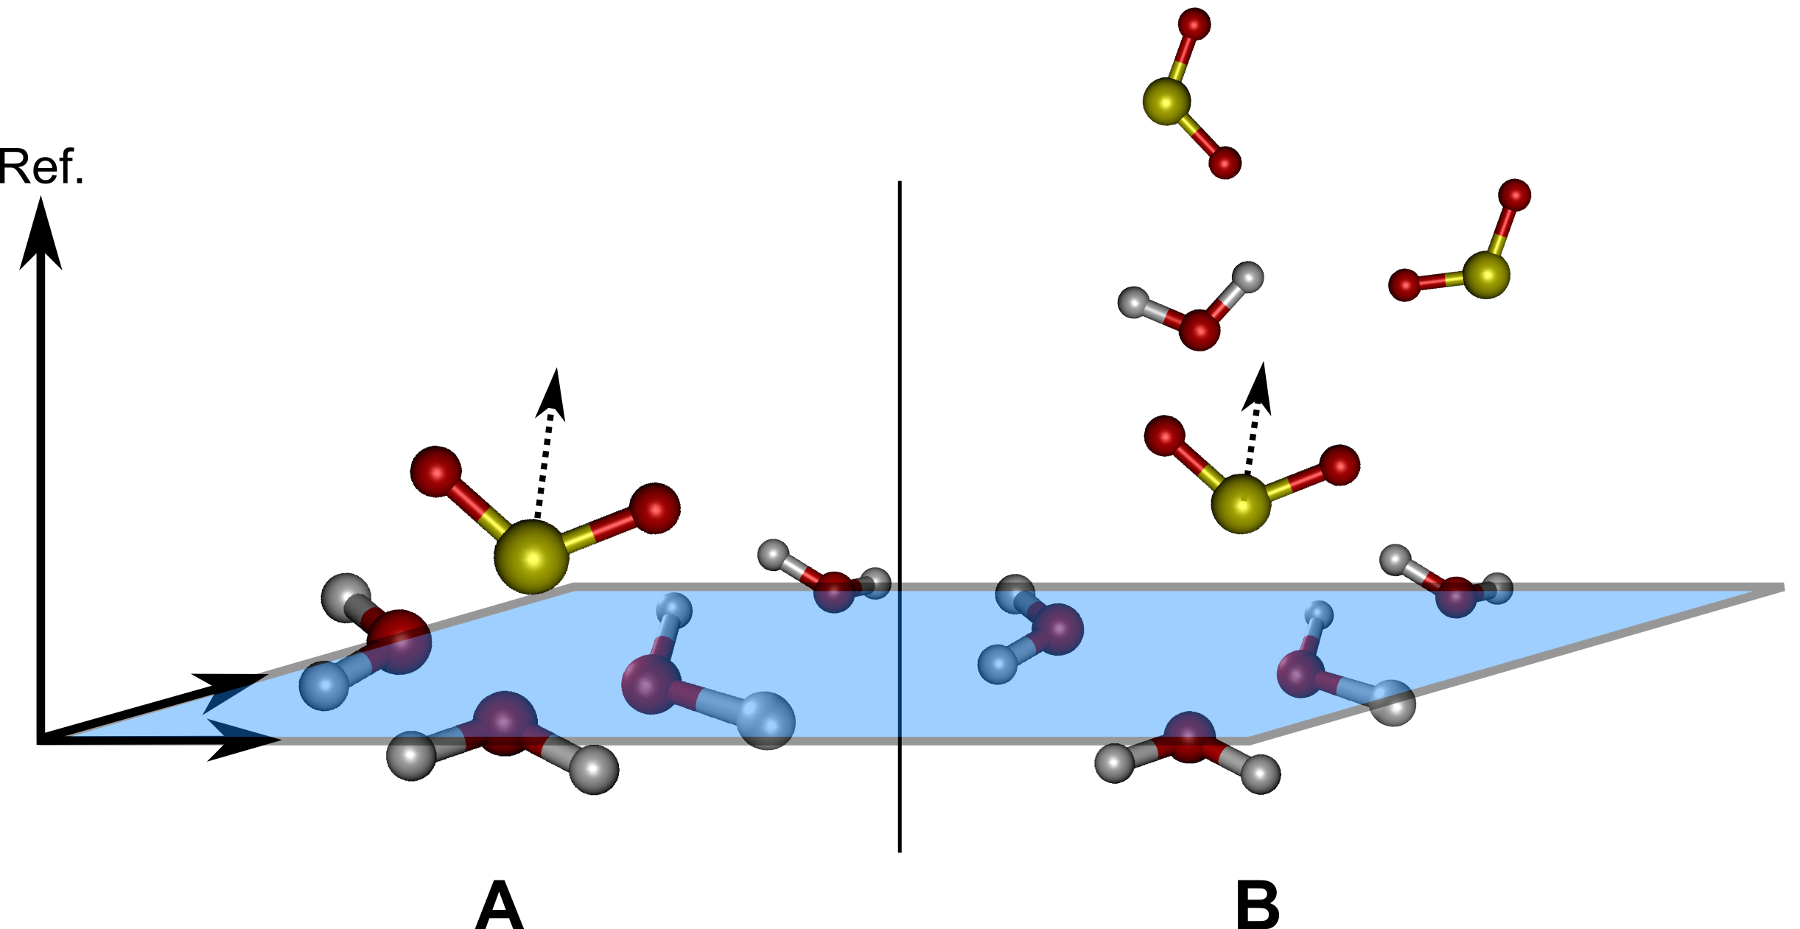
\includegraphics[scale=1.0]{images/angle-cartoons/system-surface.png}
		\caption{\wat~and \suldiox~both exhibit preferred orientations in the region near the liquid-gas interface. The neat-water system (A) with a single \suldiox~molecule (low-concentration) has surface waters orienting mostly flat to the interface. When the \suldiox~concentration is increased, as in the saturated system (B), the waters at the surface behave similar to the neat-water interface, but waters that venture into the adsorbed \suldiox~gas layer orient strongly with their bisectors pointing out from the aqueous phase towards the gas. In both cases, the \suldiox~orients with its molecular bisector pointing out to the gas phase when it is near the surface, and isotropically further into the gas phase. Sulfur, oxygen and hydrogen atoms are colored yellow, red, and white, respectively.}
		\label{fig:so2-surface-cartoon}
	\end{center}
\end{figure}

Steered molecular dynamics simulations were used to model the behavior of an adsorbing \suldiox~as it moves from the gas phase above the water down through the surface and into the bulk. The results for the transit through the interface show that in both systems of low and high \suldiox~concentration an adsorbing \suldiox~has very similar orientation to those already bound to the water surface. The \suldiox~reorients as it makes its first contact with the water surface. Within 5 $\AA$ of the surface the \suldiox~is mostly oriented with its sulfur towards the water phase. The \suldiox~pulled further into the water bulk retains its orientation until it is past the interfacial region and then isotropically orients with the bulk water.

Having now examined this passageway of \suldiox~from the gas to adsorbed aqueous phases, we may turn to further filling in the details of adsorption and interfacial chemistry of gas molecules. What species form during the adsorption transition, and how do molecular properties affect the process? Can we form a theory that will more fully explain the transit of many small molecules of environmental and industrial interest? This study is one of several aiming to characterize \suldiox~adsorption and behavior on aqueous surfaces. We plan to report further results of ongoing computational simulation and experimental studies regarding temperature and chemical constituent effects on atmospherically relevant water surfaces.


\bibliography{bib/SulfurDioxideText}

\end{document}
